% Kiosk manual - Top level
% Written by Christopher Thomas.

\documentclass[letterpaper,11pt]{report}
\usepackage[letterpaper]{geometry}
\usepackage{graphicx}
\usepackage{verbatim}
\usepackage{float} % Needed for capital H option.

\geometry{nohead,footskip=0.3in,margin=0.75in}

% Force my paragraph style, darnit.
\usepackage{indentfirst}
\setlength{\parskip}{\baselineskip}

% Custom macros.
\newcommand{\fixme}[1]{\textbf{FIXME: #1}}

% Document body.
\begin{document}

% Title page.

\pagestyle{empty}

\begin{center}
%
\vspace*{1in}
{\Huge \bfseries Kiosk User Guide} \\
{\footnotesize Written by Christopher Thomas -- \today.} \\
%
\vspace*{1in}
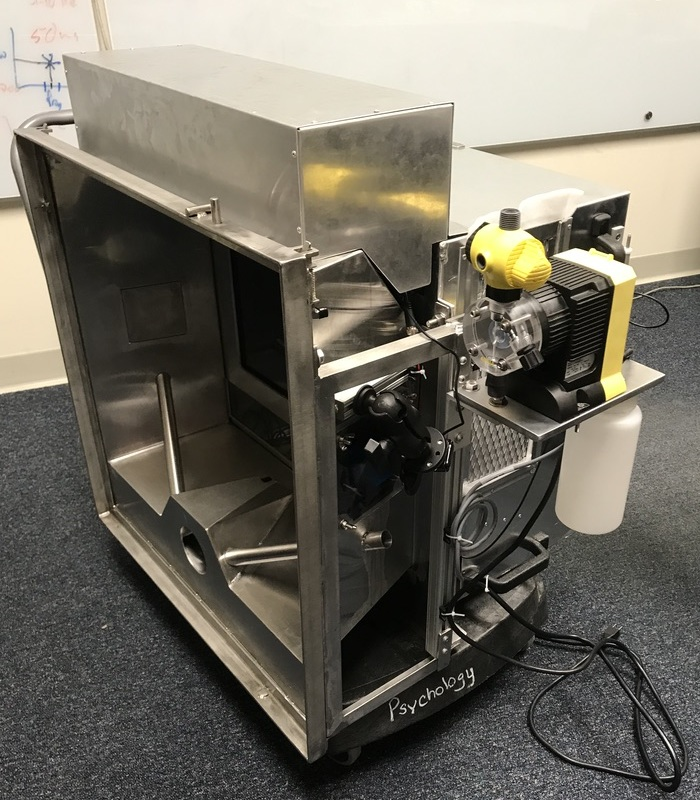
\includegraphics[width=0.7\columnwidth]
{photos/install-20181106/cover-front.jpg}
%
\end{center}
%
\clearpage
%
\pagestyle{plain}
\pagenumbering{roman}
\setcounter{page}{1}
%
\tableofcontents
%
\clearpage
\pagestyle{plain}
\setcounter{page}{1}
\pagenumbering{arabic}
% NOTE - "\thispagestyle" is used for part and chapter beginning pages,
% and overrides \pagestyle. Redefine it to be harmless.
\renewcommand{\thispagestyle}[1]{}

% Not using "parts" for now; just chapters.

% Daily use, and accessories (if we make any).
% Kiosk manual - Routine activities.
% Written by Christopher Thomas.

\chapter{Routine Activities}
\label{sect-routine}

\section{Startup and Shutdown}
\label{sect-routine-startupdown}

To power on the electronics bay equipment:

\begin{itemize}
%
\item Turn on the leftmost power bar, and check that the rightmost one
(plugged into the left bar) is also turned on.
%
\item Check that the fans have spun up. They should turn on within a few 
seconds of receiving power.
%
\item Check that the wireless gateway is on (there should be visible lights 
blinking).

If there are no lights, check that the gateway's power button is 
turned on (if it has one). This is the \textbf{large, exposed} button - do 
not press any small or inset buttons (those either reset the gateway to 
default settings or tell it to use an insecure reconfiguration method - 
both are bad).
%
\item Press and hold the NeuroCam machine's power button until it lights up
and the machine's fan spins up.

This should only take about a second. Do not hold it for longer than 3
seconds - holding it 4 seconds or longer forces an immediate shutdown, which
can cause corruption.
%
\item Press and hold the Unity machine's power button until it lights up and
the machine's fan spins up.

Per previous entry, this should only take about a second.
%
\item Check that the small monitor and the touch screen are both showing
a Windows boot or login screen.

If either one is not showing a screen, check that it's powered on.
%
\item Check that you can access the NeuroCam gateway, and that you can
access the NeuroCam's control web page.

The NeuroCam takes 30-60 seconds to boot, so be sure to leave sufficient
time before accessing it.
%
\item Once everything's running properly, close and lock the electronics 
bay doors.
%
\end{itemize}

\clearpage
To safely shut down the electronics bay equipment:

\begin{itemize}
%
\item Log in to the NeuroCam's web page over the wireless network. Click
the ``shutdown'' button.
%
\item Check that the NeuroCam's power light turns off. This may take
several seconds.

\begin{itemize}
\item If the NeuroCam does not power off, it can be forced to power down by
pressing and holding the power button for 4-5 seconds.

\textbf{NOTE} - This may cause data corruption and other problems, so try to
avoid this if possible.
\end{itemize}
%
\item If the Unity machine is logged in:
\begin{itemize}
\item \fixme{key sequence for power-off goes here}.
\end{itemize}
%
\item If the Unity machine is not logged in:
\begin{itemize}
\item Press a harmless key (such as ``shift'') to wake up the display.
\item Press ``tab'' until the power icon is highlighted (this will take 
multiple keystrokes).
\item Hit ``enter'' to expand the power menu.
\item Use the up and down cursor keys to highlight ``Shut Down''.
\item Hit ``enter''.
\end{itemize}
%
\item Check that the Unity machine's power light turns off. This may take
several seconds.

\begin{itemize}
\item If the Unity machine does not power off, it can be forced to shut down
per above. This may cause data corruption and other problems, as noted.
\end{itemize}
%
\item Locate the power switch on the left power bar (the one whose cord
goes outside), and turn it off.
%
\item Once everything's shut down, close and lock the electronics bay doors.
%
\end{itemize}

%
% This is the end of the file.

% Kiosk manual - Installation and setup.
% Written by Christopher Thomas.

\chapter{Kiosk Setup}
\label{sect-setup}

\section{Checklist}
\label{sect-setup-checklist}

First-time kiosk setup involves assembling fittings on the kiosk housing 
and installing and cabling electronic equipment inside the electronics bay.
A summary of the steps involved is shown below; photographs and additional
notes are given in Section \ref{sect-setup-howto}.
A cabling diagram for the kiosk is shown in Figure \ref{fig-kiosk-cabling}.

Initial mechanical work:
\begin{itemize}
\item Separate the kiosk face from the electronics bay.
\item With the kiosk face:
\begin{itemize}
\item Remove the outer viewport window from ports that will have cameras
installed.
\item Remove both viewport windows from the port that will have the
cleaning hatch installed.
\item Remove the pump bracket from the side which has the cleaning port.
\item Install the cleaning hatch in its port.
\item Install the pump mounting plate on the remaining pump bracket. The pump
is away from the face of the kiosk, towards the direction of the electronics
bay.
\item Install light filter plates on the viewport windows that will have
cameras. The synchronization LEDs should be close to the camera mounting
arms.
\end{itemize}
\item With the electronics bay:
\begin{itemize}
\item Remove internal shelves.
\item Remove ventilation grilles.
\item Remove fan dummy panels from either the top level or both levels
(for mounting two or four fans, respectively).
\item Remove the external wiring panel from the side nearest the pump.
\item Remove the monitor tray.
\item Seat the touch screen in the monitor tray. Annotate the back of the
monitor tray to show connector locations.
\item Install the monitor and tray in the electronics bay.
\item Install the fans and fan guards.
\item Line the ventilation grilles with HVAC tape to render them glove-safe.
\item Cut filter pads and install the ventilation grilles with filters in
the electronics bay.
\end{itemize}
\end{itemize}

Electronics work:
\begin{itemize}
\item \textbf{NOTE} - This does not include eye-tracker installation.
Power cabling is placed in the eye-tracker bay.
\item \textbf{NOTE} - During each cabling step, excess cable length should
be coiled and zip-tied, and routed cables should be zip-tied to cable mounts
where appropriate.
\item Install power distribution bars at the bottom of the bay (turned off).
\item Reinstall bay shelves.
\item Install fan power plug and connect fans.
\item Install touch screen power supply. Connect power, display, and USB
cables to the touch screen.
\item Install small monitor, keyboard, and mouse on the right-hand side of
the middle shelf. Install monitor power supply in the bottom of the bay.
Route data cables to the top shelf.
\item Install router with two ethernet cables connected to LAN ports on the
left-hand side of the middle shelf. Install router power supply in the 
bottom of the bay. Route ethernet cables to the top shelf. Ensure that the
router's power switch is turned on, if it has one.
\item Install Neurarduino on the top shelf, left-hand side.
\item Install pump reward box on the top shelf, left-hand side. Cable the
pump reward box to the Neurarduino.
\item Install pump reward fob. Use hook-and-loop cable ties to hang it from
the electronics bay carrying handle on the pump side of the unit. Cable the
fob to the pump reward box.
\item Install the Unity machine's power supply in the bottom of the bay.
Route it to the left-hand side of the top shelf.
\item Install Unity machine on top of the Neurarduino. Attach Unity machine
cable connections (which should already be routed to the top shelf).
\item Install LED box on the top shelf, right-hand side. Route BNC cables 
from the LED box out appropriate camera cabling ports; do not coil the 
LED BNC cables yet.
\item Install the NeuroCam machine's power supply in the bottom of the bay.
Route it to the right-hand side of the top shelf.
\item Install NeuroCam and NeuroCam USB hub. Cable the LED box to the
USB hub and the USB hub to the NeuroCam. Attach the NeuroCam power and
ethernet cables.
\end{itemize}

Electronics tests:
\begin{itemize}
\item Turn on power bar. Press power switches on Unity and NeuroCam
computers. Wait 60 seconds for machines to boot.
\item Check that the Unity machine's login display is shown on the touch 
screen and on the small monitor.
\item Check that an authorized machine can connect to the NeuroCam via the
kiosk's router.
\item Perform graceful shutdowns of the Unity machine and NeuroCam machine.
\item Turn off power bar.
\end{itemize}

Final mechanical work:
\begin{itemize}
\item Reattach the kiosk face to the electronics bay.
\item Install cameras.
\item Screw pump control cable on to pump. Use pliers for this.
\item Install pump.
\item Connect LED BNC cables to camera port LEDs. Coil and zip-tie excess 
cabling \textit{inside} the electronics bay. Do \textbf{not} zip-tie BNC
cables to the kiosk face exterior frame unless this is unavoidable. If it
is unavoidable, keep the zip-ties loose enough that they can be cut without
damaging the BNC cables.
\item Connect camera USB cables to the NeuroCam computer. Coil excess
cabling \textit{inside} the electronics bay. Zip-tie the coils, but do
\textbf{not} zip-tie the coils or cables to cable mounts (it must be possible
to disconnect and withdraw the camera USB cables). Exterior camera cables
may be zip-tied to the kiosk face's frame.
\item Connect the pump control cable to the pump box. Coil excess cabling
\textit{inside} the electronics bay. Zip-tie the coils, but do \textbf{not}
zip-tie the coils or cables to cable mounts (it must be possible to
disconnect and withdraw the pump control cable).
\item Zip-tie cables that pass through the lower exterior cable entry port
to the adjacent handle. Keep this loose enough that it can be cut without
damaging the cables.
\item Replace camera cover.
\item Install pump hoses.
\item Mount the kiosk so that the underside is accessible.
\item Install sipper tube.
\item Make remaining pump hose connections.
\end{itemize}

\begin{figure}[h]
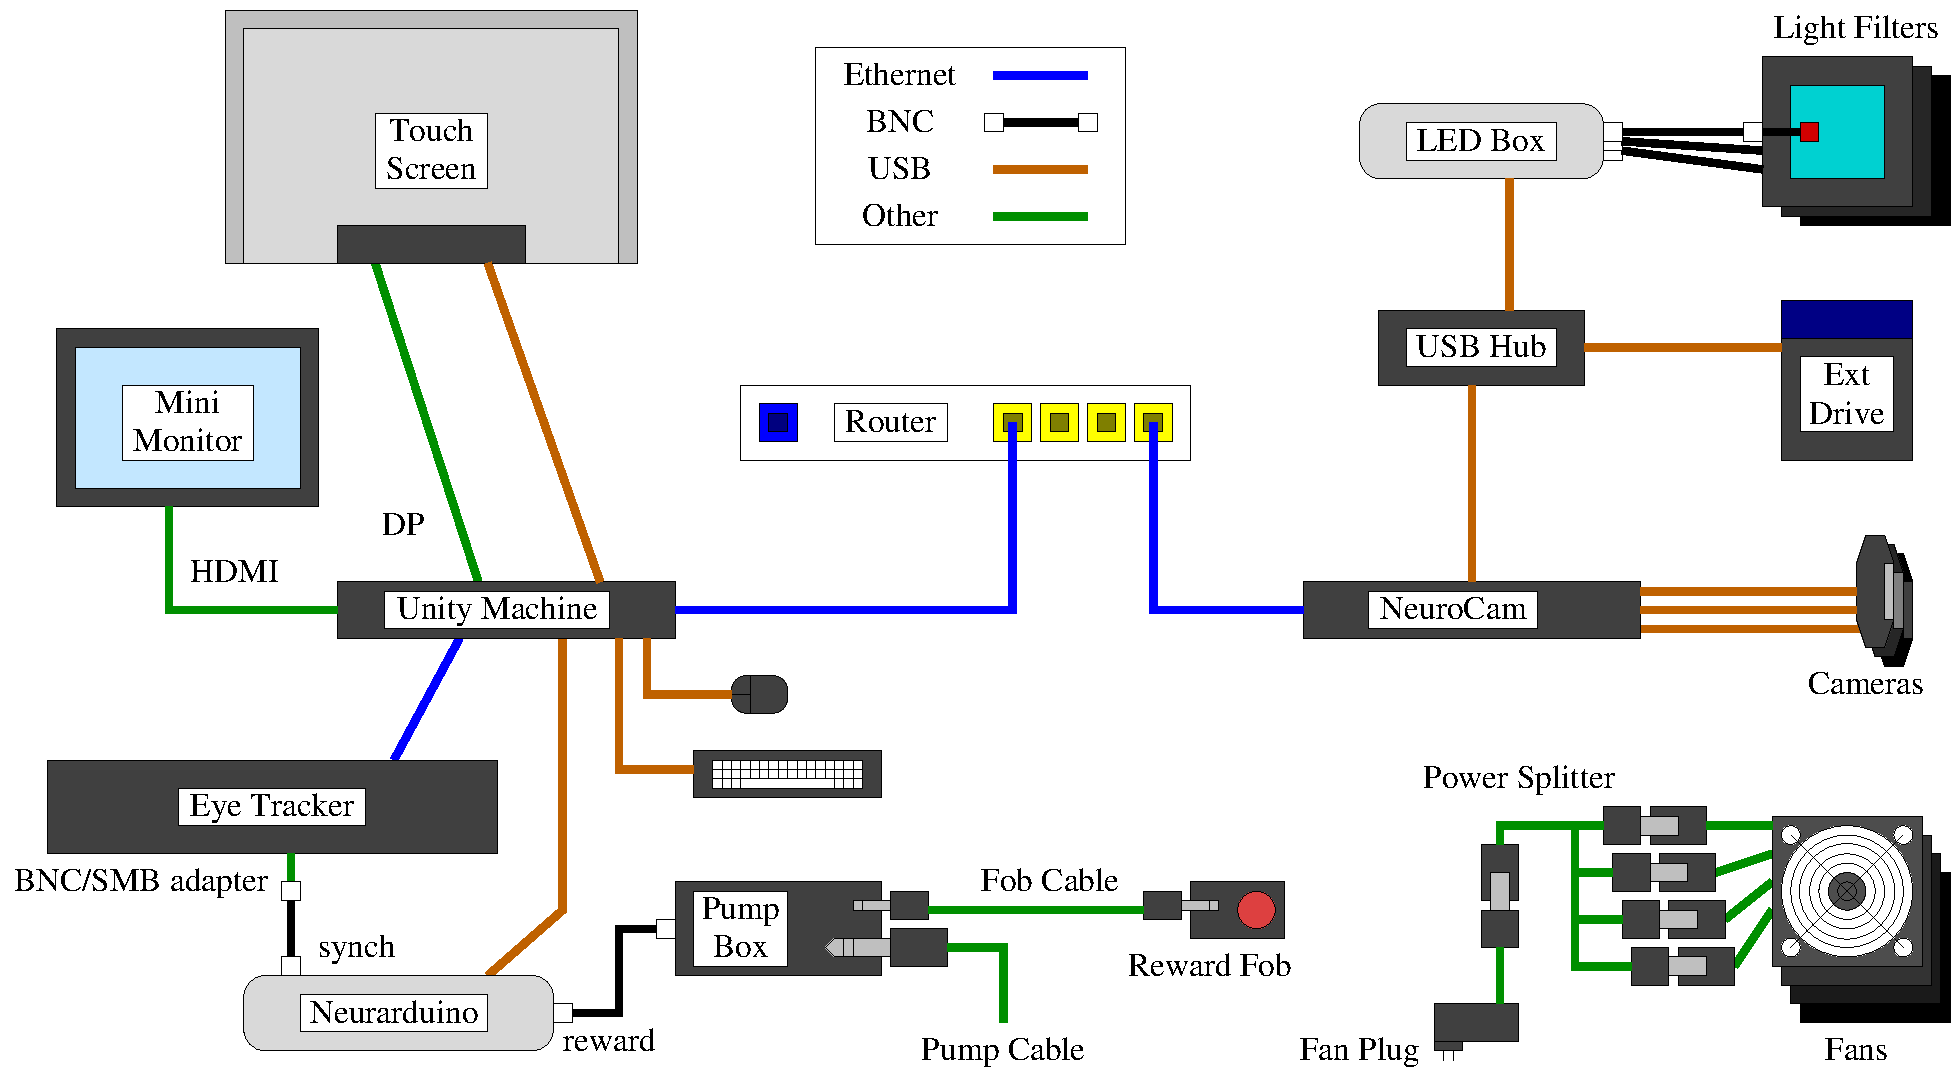
\includegraphics[width=0.99\columnwidth]{cabling/kiosk-cabling-2019.pdf}
\caption{Kiosk cabling daigram.}
\label{fig-kiosk-cabling}
\end{figure}

\clearpage
\section{Kiosk Assembly Notes}
\label{sect-setup-howto}

%
%
\subsection{Viewports and Hatch}
\label{sect-setup-howto-viewports}

\begin{tabular}{ccc}
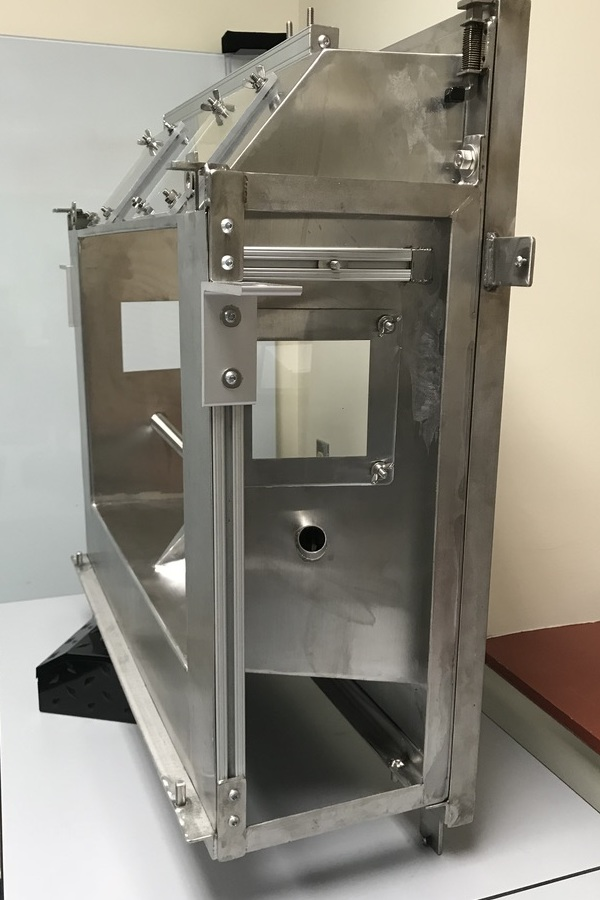
\includegraphics[width=0.4\columnwidth]
{photos/install-20181106/face-before.jpg} &
~~~ &
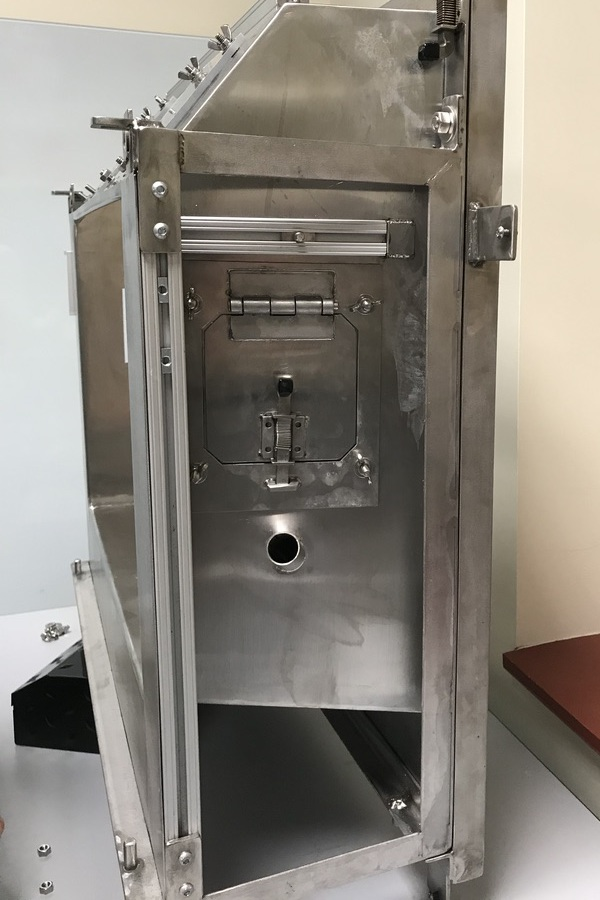
\includegraphics[width=0.4\columnwidth]
{photos/install-20181106/hatch.jpg} \\
\end{tabular}

%
%
\clearpage
\subsection{Light Filters and Cameras}
\label{sect-setup-howto-lightfilt}

The LEDs should be as close as possible to the camera mounts. The cameras
must have LEDs in their field of view when in their final positions.

\begin{tabular}{ccc}
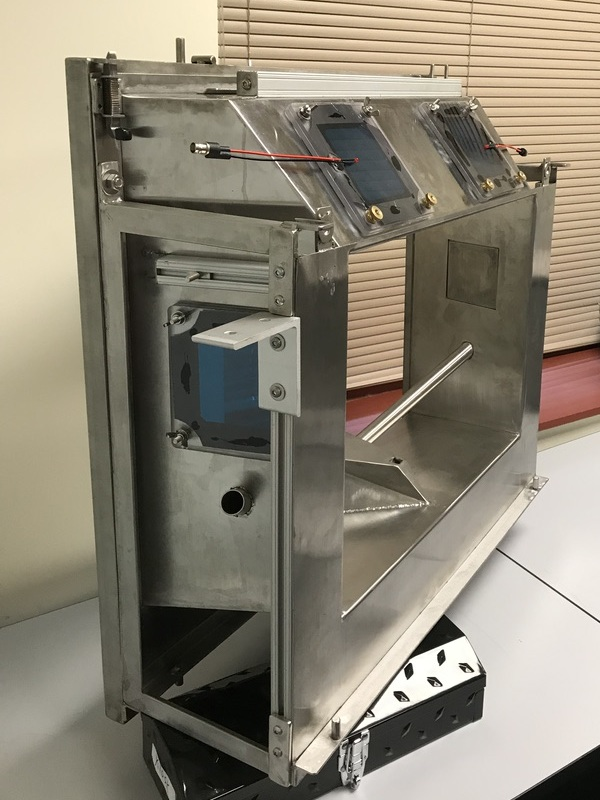
\includegraphics[height=0.55\columnwidth]
{photos/install-20181106/lightfilts.jpg} &
~~~ &
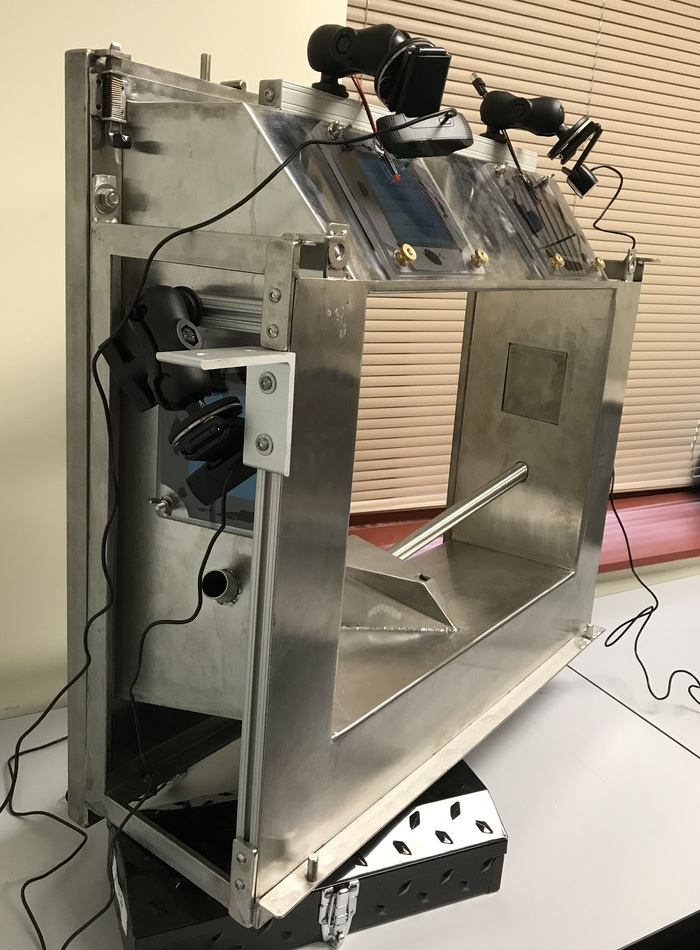
\includegraphics[height=0.55\columnwidth]
{photos/install-20181106/cameras.jpg} \\
\end{tabular}

%
%
\clearpage
\subsection{Electronics Bay Prep}
\label{sect-setup-howto-bay}

\begin{tabular}{ccc}
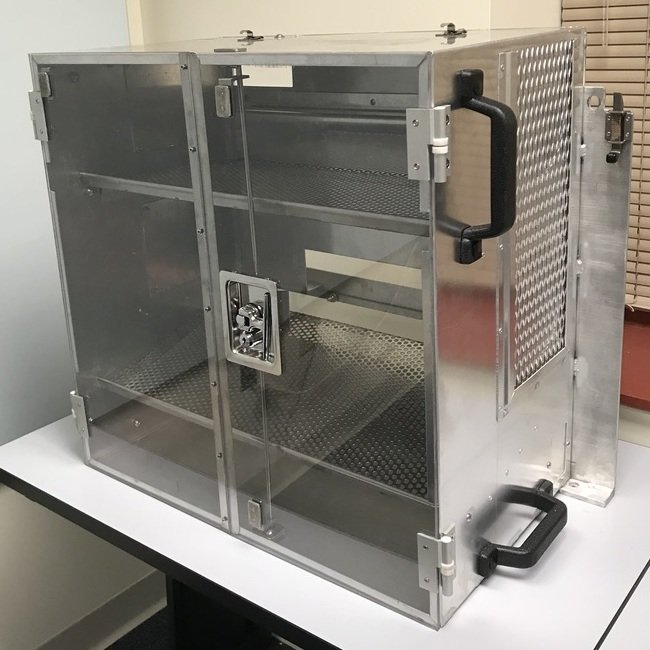
\includegraphics[width=0.4\columnwidth]
{photos/install-20181106/bay-before.jpg} &
~~~ &
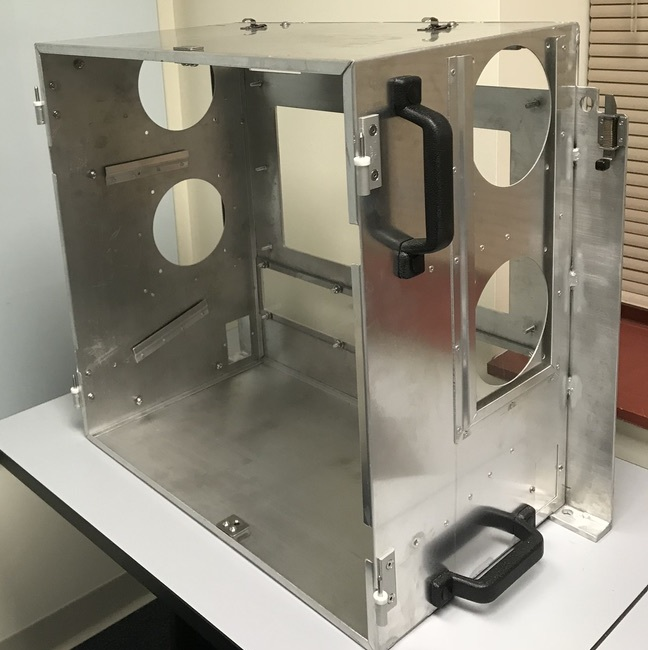
\includegraphics[width=0.4\columnwidth]
{photos/install-20181106/bay-stripped.jpg} \\
 & ~ & \\
\multicolumn{3}{c}{%
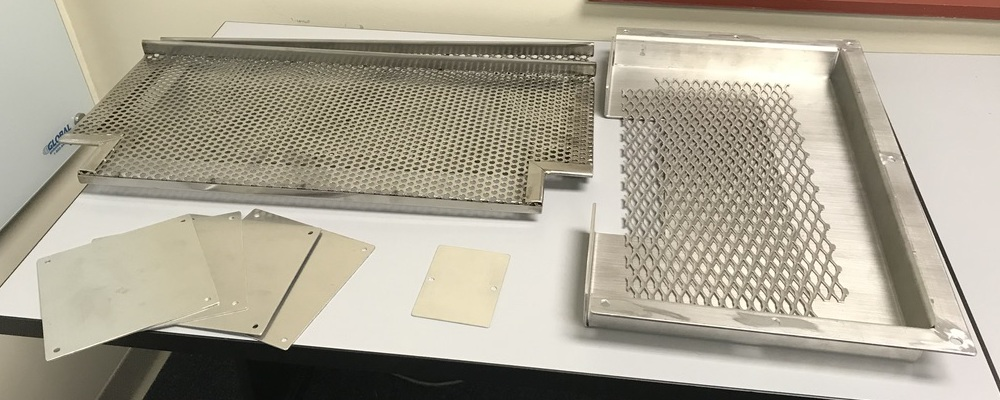
\includegraphics[width=0.85\columnwidth]
{photos/install-20181106/bay-parts.jpg}%
} \\
\end{tabular}

%
%
\clearpage
\subsection{Touch-Screen Tray}
\label{sect-setup-howto-touch}

\begin{tabular}{ccc}
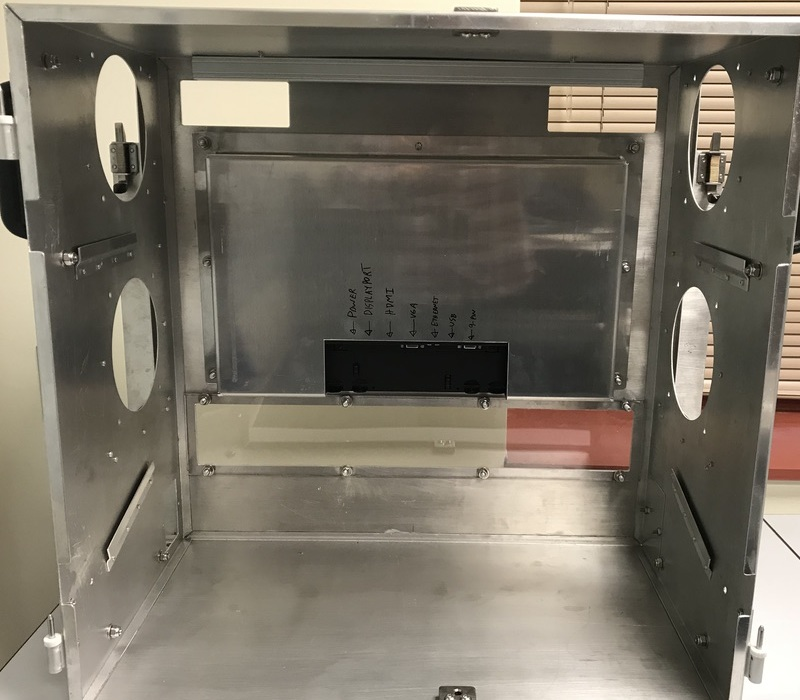
\includegraphics[height=0.45\columnwidth]
{photos/install-20181106/ts-installed.jpg} &
~~~ &
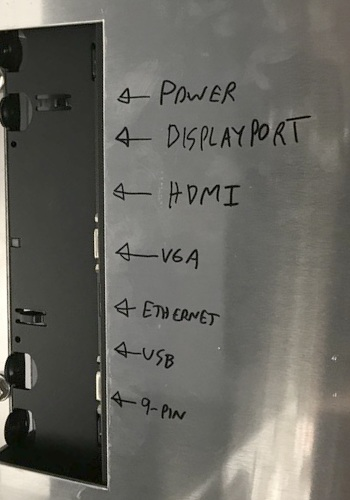
\includegraphics[height=0.45\columnwidth]
{photos/install-20181106/ts-labels.jpg} \\
\end{tabular}

%
%
\clearpage
\subsection{Fans}
\label{sect-setup-howto-fans}

The photographed version of the kiosk needed adapter plates to mount the
fans. Later versions mount the fans directly to the electronics cabinet.

\textbf{NOTE} - Fans on one side blow into the electronics bay (intake fans),
and fans on the other side blow out of the electronics bay (exhaust fans).
One pair of fans has the stickers facing in and one pair has the stickers
facing out.

\begin{center}
\begin{tabular}{ccc}
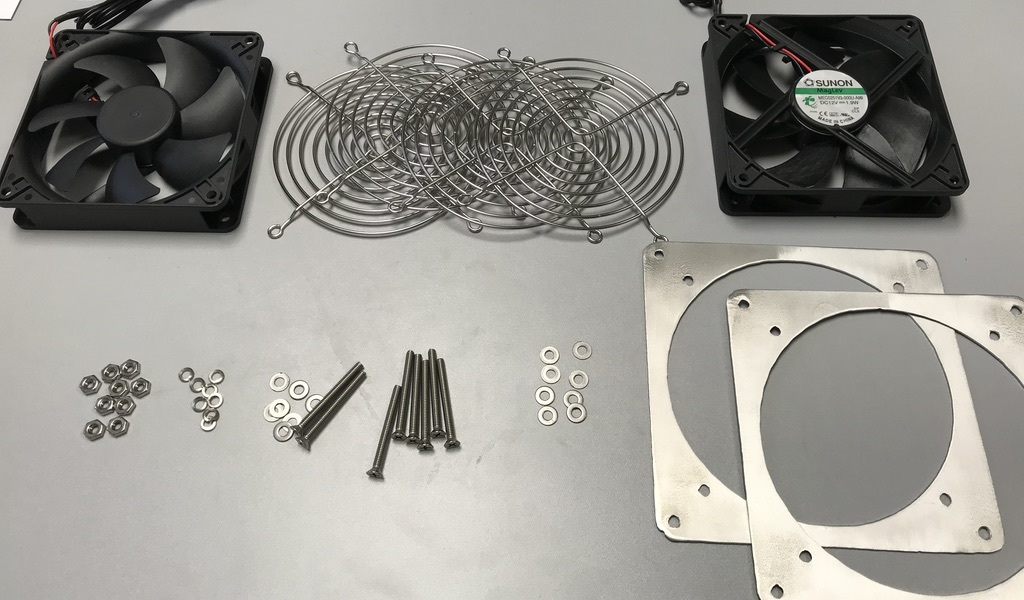
\includegraphics[height=0.3\columnwidth]
{photos/install-20181106/fan-parts.jpg} &
~~~ &
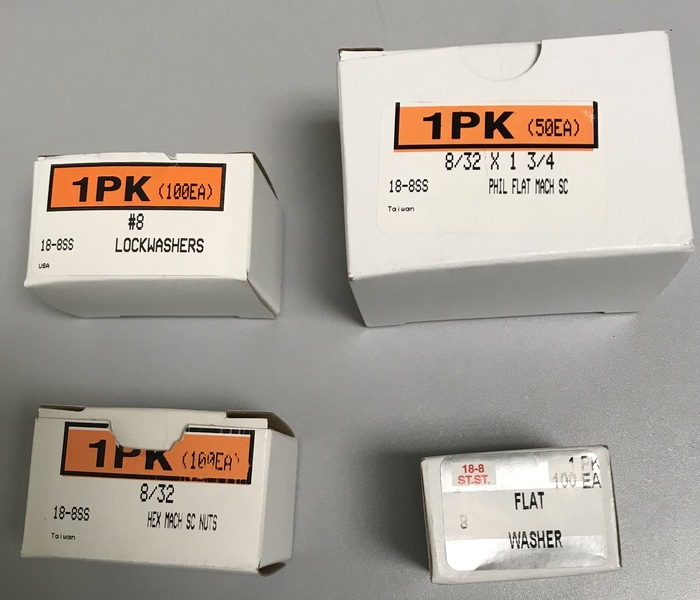
\includegraphics[height=0.3\columnwidth]
{photos/install-20181106/fan-screws.jpg} \\
\end{tabular}

\begin{tabular}{ccc}
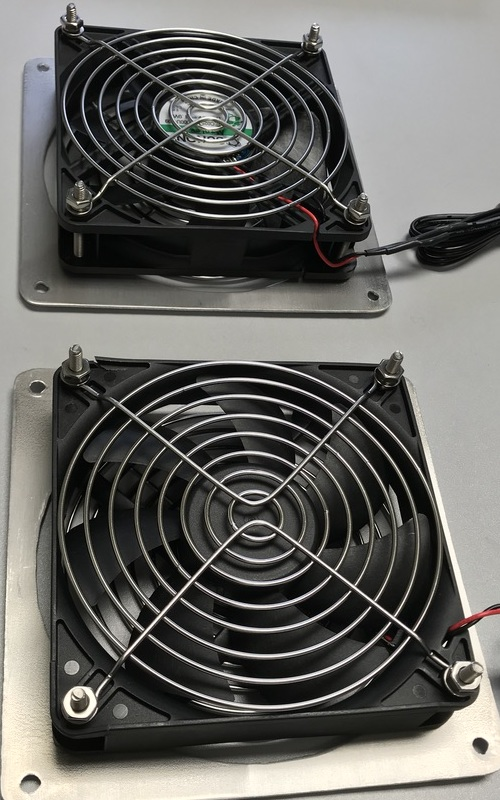
\includegraphics[height=0.6\columnwidth]
{photos/install-20181106/fan-assembled.jpg} &
~~~ &
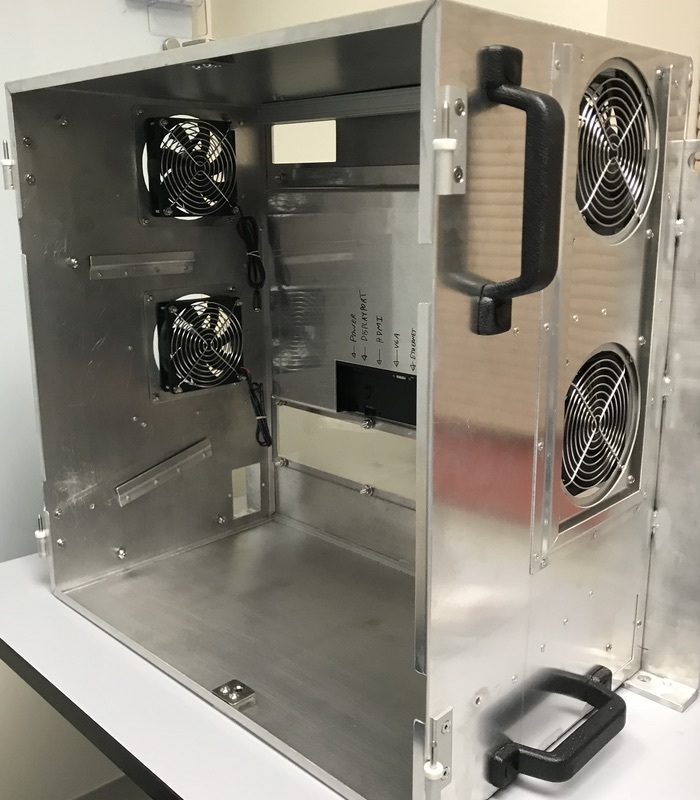
\includegraphics[height=0.6\columnwidth]
{photos/install-20181106/fan-installed.jpg} \\
\end{tabular}
\end{center}

%
%
\clearpage
\subsection{Air Filters}
\label{sect-setup-howto-airfilt}

\begin{tabular}{ccc}
\multicolumn{3}{c}{%
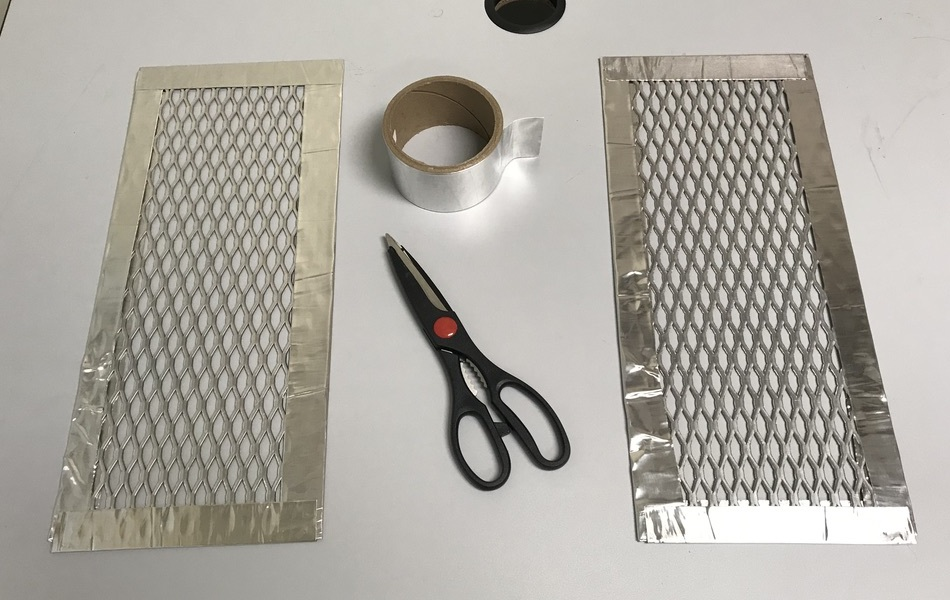
\includegraphics[height=0.5\columnwidth]
{photos/install-20181106/air-taped.jpg}%
} \\
 & ~ & \\
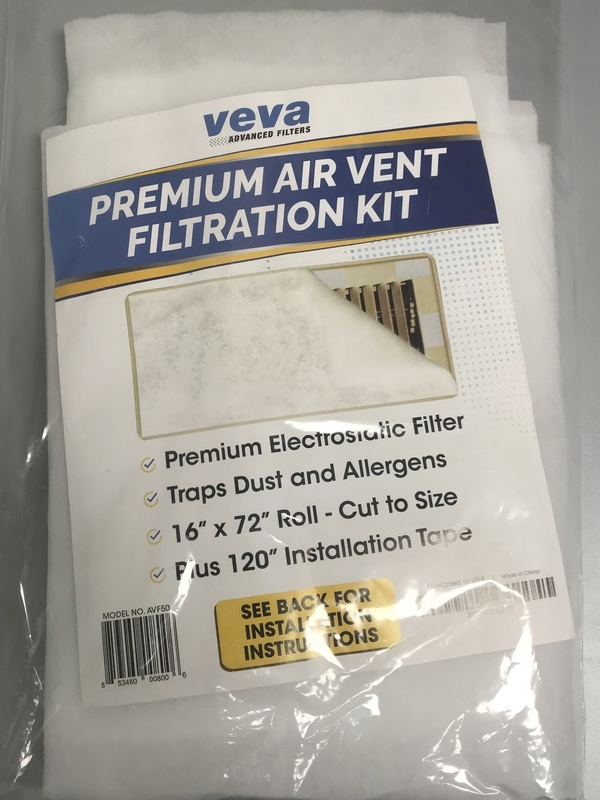
\includegraphics[height=0.5\columnwidth]
{photos/install-20181106/air-batting.jpg} &
~~~ &
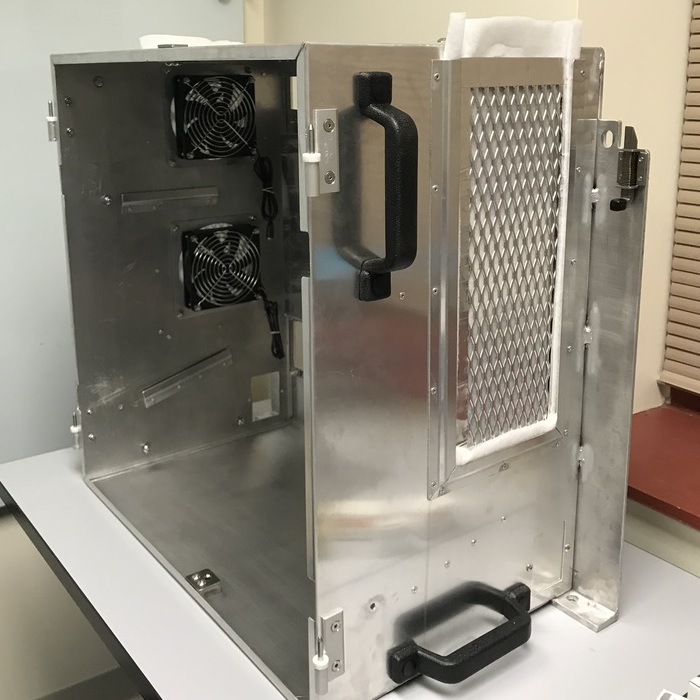
\includegraphics[height=0.5\columnwidth]
{photos/install-20181106/air-installed.jpg} \\
\end{tabular}

%
%
\clearpage
\subsection{Power Bars and Shelves}
\label{sect-setup-howto-power}

\textbf{NOTE} - The eye-tracker is not installed in the photographed version
of the kiosk. Power cabling is placed in the eye-tracker bay.

\begin{center}
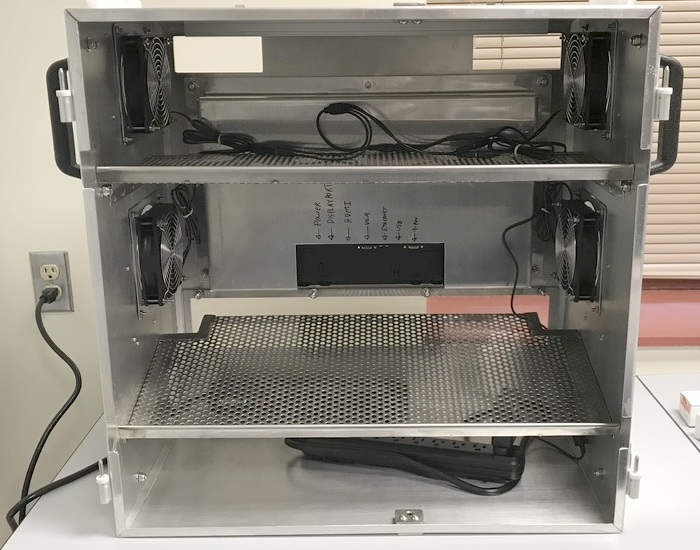
\includegraphics[width=0.9\columnwidth]
{photos/install-20181106/power.jpg}
\end{center}

%
%
\clearpage
\subsection{Small Monitor, Keyboard, and Mouse}
\label{sect-setup-howto-smallmon}

\textbf{NOTE} - The setup photographed did not have a mouse at the time of
installation. A keyboard with integrated touchpad or other pointing device
may be preferable.

\begin{center}
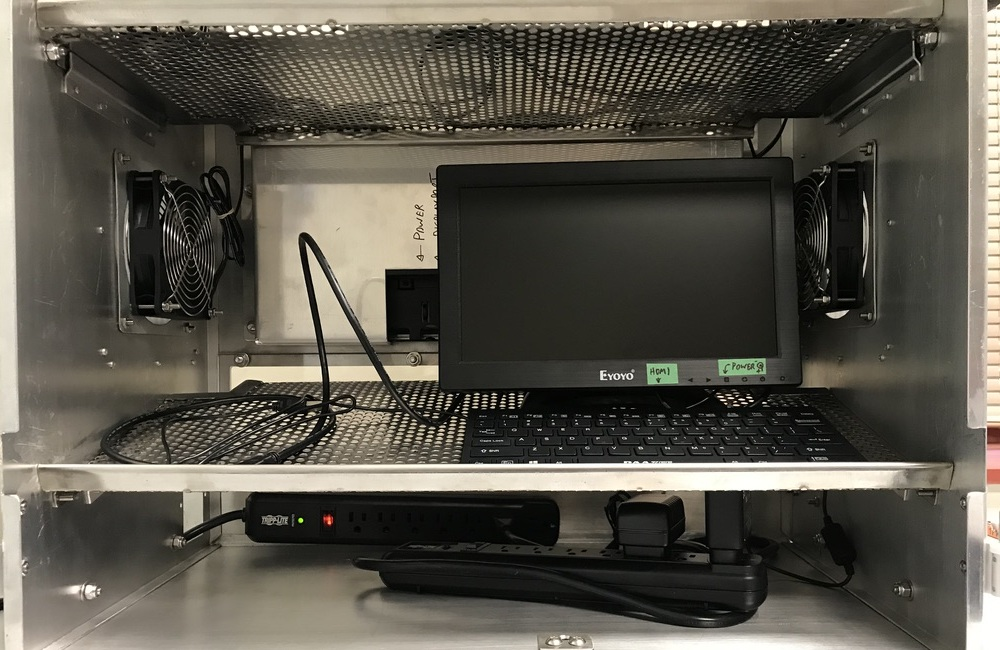
\includegraphics[width=0.9\columnwidth]
{photos/install-20181106/small-mon.jpg}
\end{center}

%
%
\clearpage
\subsection{Wireless Gateway}
\label{sect-setup-howto-router}

\textbf{NOTE} - The antennae for the wireless gateway should be far away
from the metal walls, and nearby cabling should never run parallel to the
antennae.

\begin{center}
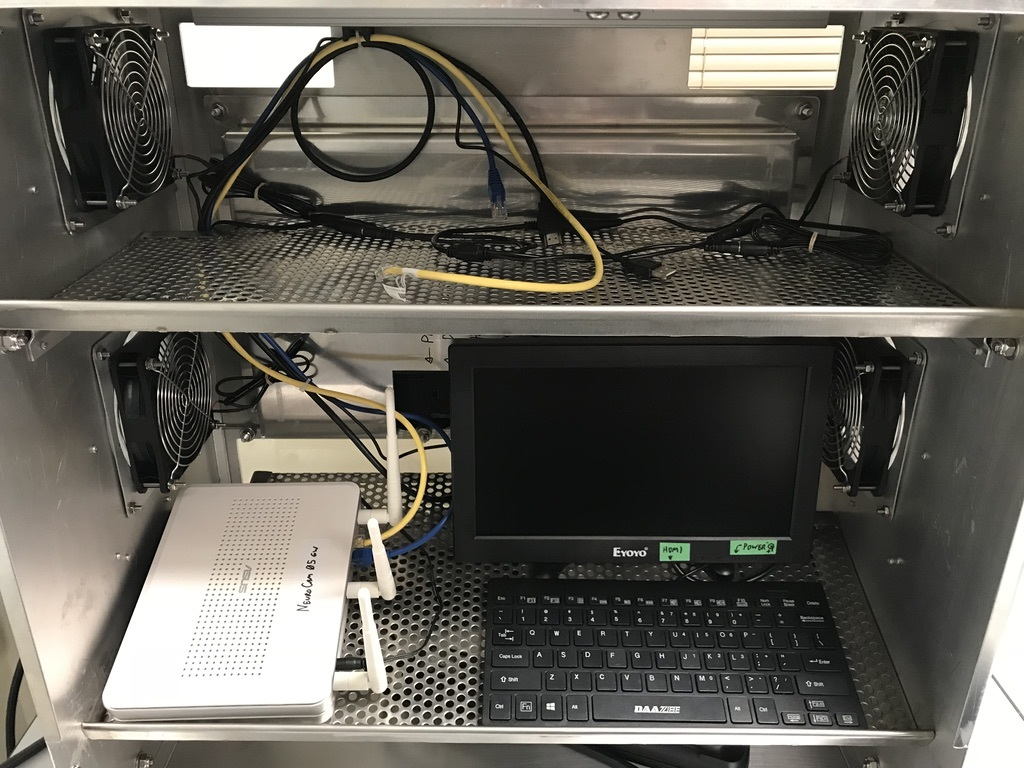
\includegraphics[width=0.9\columnwidth]
{photos/install-20181106/small-mon-gateway.jpg}
\end{center}

%
%
\clearpage
\subsection{Neurarduino and Pump Control Box}
\label{sect-setup-howto-ard}

\begin{center}
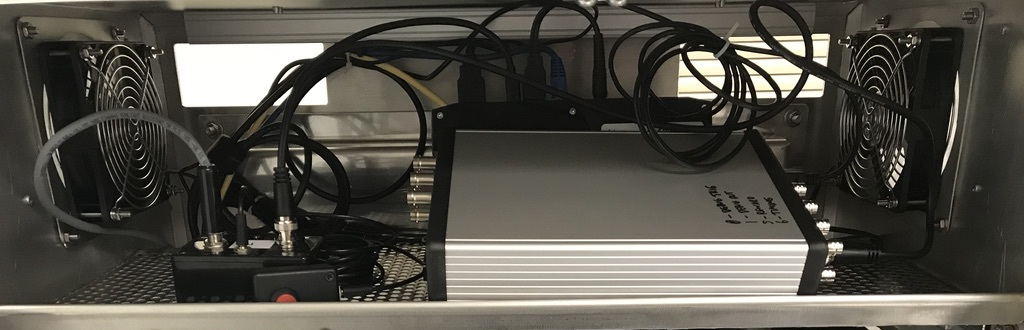
\includegraphics[width=0.9\columnwidth]
{photos/install-20181106/ard-pbox-wiring.jpg}
\end{center}

%
%
\subsection{Unity Machine}
\label{sect-setup-howto-unity}

\begin{center}
\begin{tabular}{c}
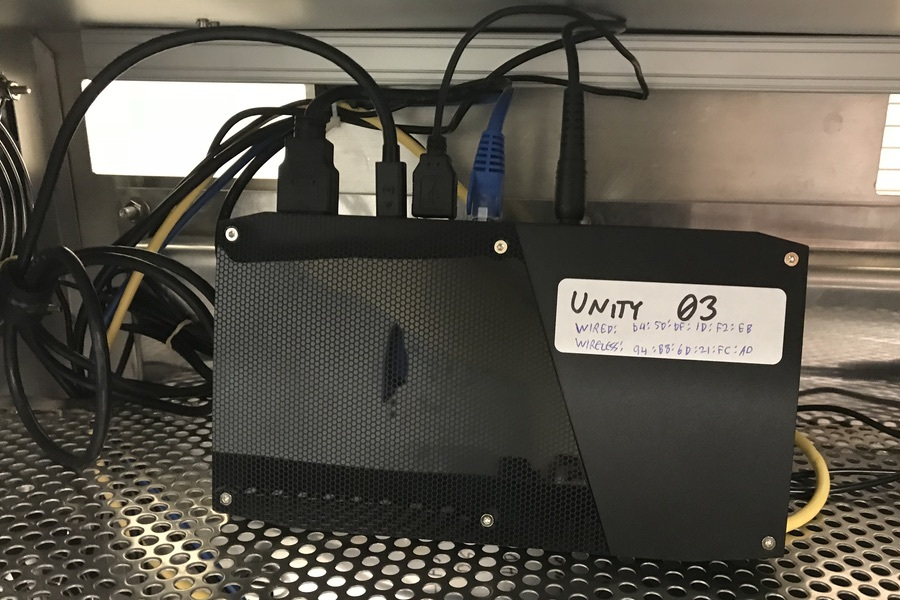
\includegraphics[width=0.6\columnwidth]
{photos/install-20181106/unity-wiring.jpg} \\
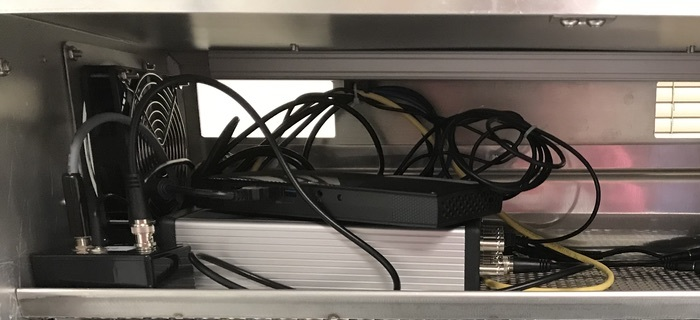
\includegraphics[width=0.8\columnwidth]
{photos/install-20181106/ard-unity-placement.jpg} \\
\end{tabular}
\end{center}

%
%
\clearpage
\subsection{LED Box}
\label{sect-setup-howto-ledbox}

\begin{center}
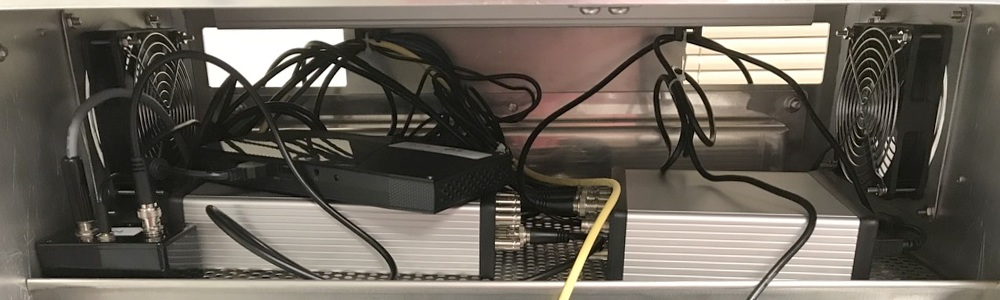
\includegraphics[width=0.9\columnwidth]
{photos/install-20181106/led-box.jpg}
\end{center}

%
%
\subsection{NeuroCam Machine}
\label{sect-setup-howto-neurocam}

\begin{center}
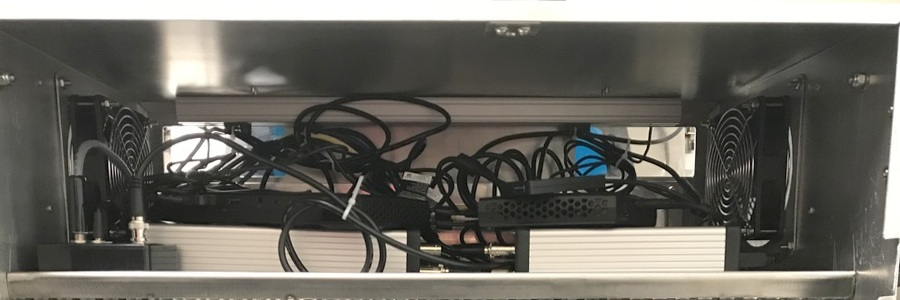
\includegraphics[width=0.9\columnwidth]
{photos/install-20181106/led-ncam-placement.jpg}
\end{center}

%
%
\clearpage
\subsection{External Cabling and Pump}
\label{sect-setup-howto-extcable}
\label{sect-setup-howto-pump}

\begin{tabular}{ccc}
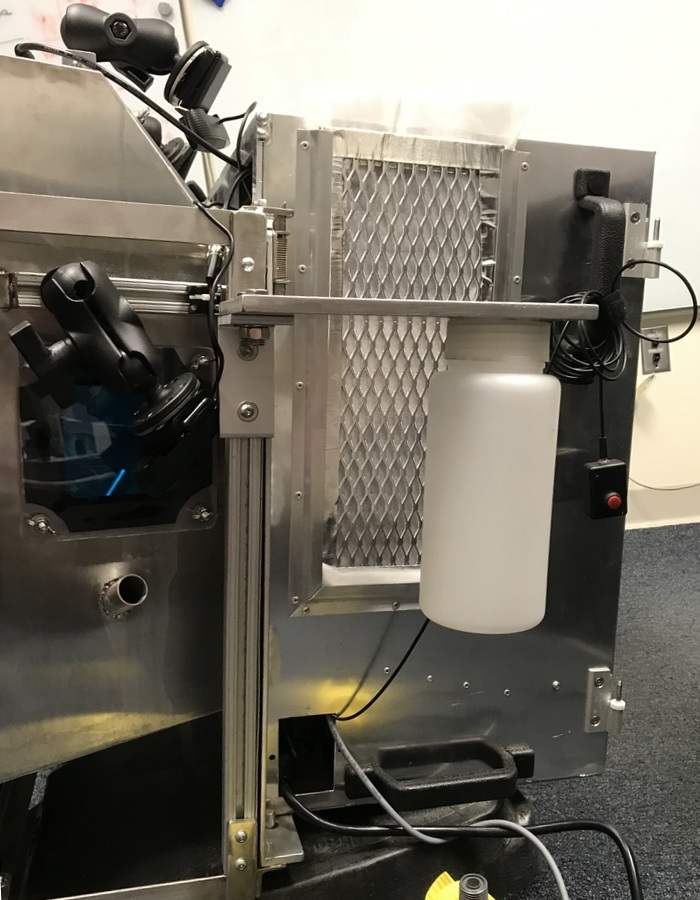
\includegraphics[height=0.5\columnwidth]
{photos/install-20181106/ext-cabling.jpg} &
~~~ &
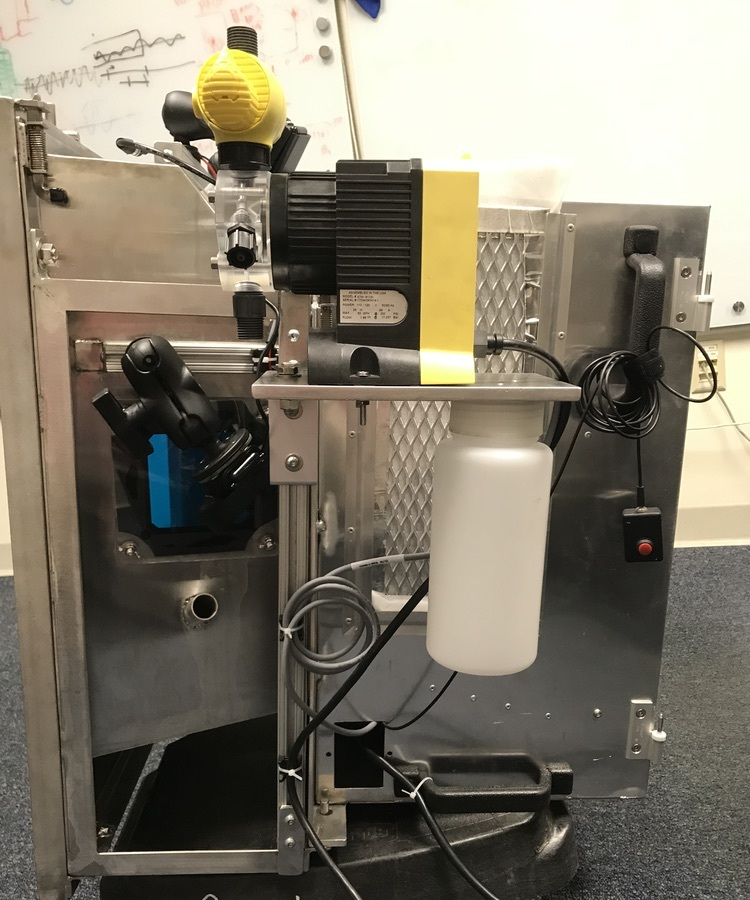
\includegraphics[height=0.5\columnwidth]
{photos/install-20181106/pump.jpg} \\
\end{tabular}

%
%
\subsection{Camera Cover}
\label{sect-setup-howto-cover}

\begin{tabular}{ccc}
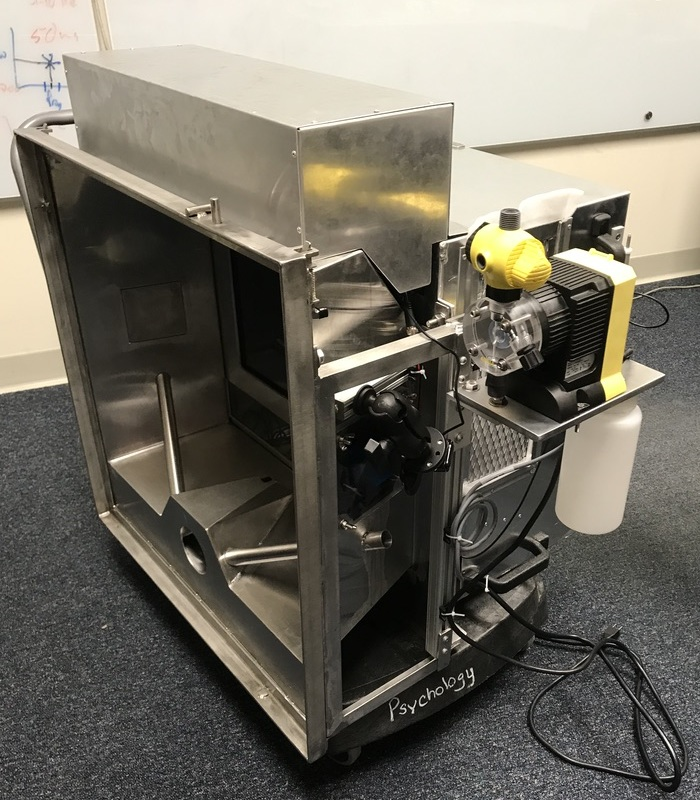
\includegraphics[height=0.47\columnwidth]
{photos/install-20181106/cover-front.jpg} &
~~~ &
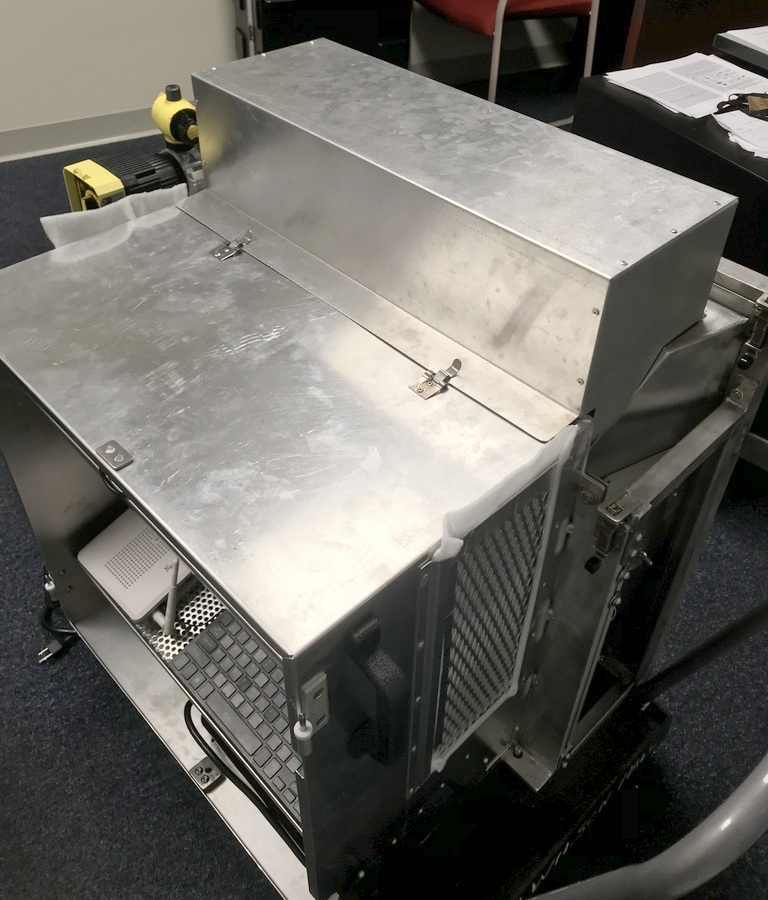
\includegraphics[height=0.47\columnwidth]
{photos/install-20181106/cover-back.jpg} \\
\end{tabular}

%
%
\clearpage
\subsection{Pump Hoses}
\label{sect-setup-howto-hoses}

\fixme{Need photos for this.}

%
% This is the end of the file.

% Kiosk manual - Pump control box.
% Written by Christopher Thomas.

\chapter{Pump Control Box}
\label{sect-pumpbox}

\section{Overview}
\label{sect-pumpbox-over}

The pump control box allows the reward pump to be controlled by a 5V
active-high signal over BNC for automated rewards and by pressing a button 
on a fob for manual rewards. A schematic for the pump control box is
shown in Figure \ref{fig-pumpbox-schem}.

\textbf{NOTE} -- While a similar 1/4'' plug is used for old and new boxes,
cable plugs wired for old control boxes are \textbf{NOT} compatible with
the current control box, and vice versa. New cables use a stereo plug with
+15~V on the ring.

A diagram of box cutouts is shown in Figure \ref{fig-pumpbox-boxes}. A bill
of materials is given in Table \ref{tab-pumpbox-bom}.

\begin{figure}[h]
\begin{center}
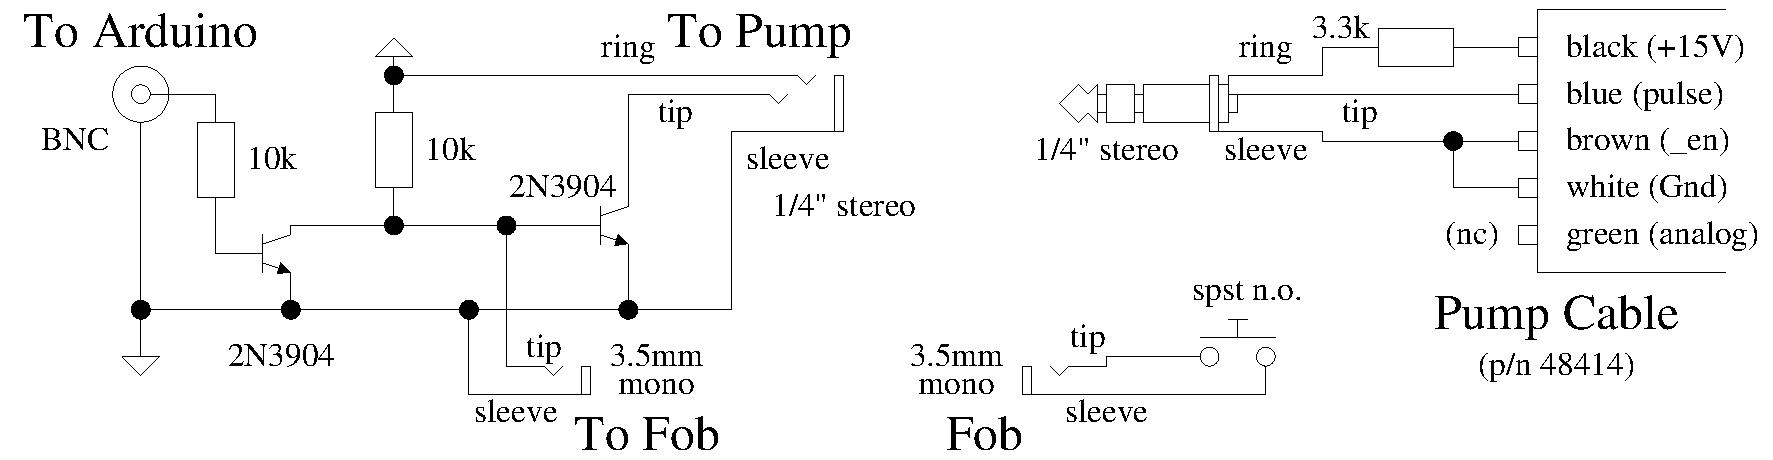
\includegraphics[width=0.95\columnwidth]
{figs-pump/pump-box-v1-schem.pdf}
\end{center}
\caption{Pump control box schematic.}
\label{fig-pumpbox-schem}
\end{figure}

\begin{figure}[h]
\begin{center}
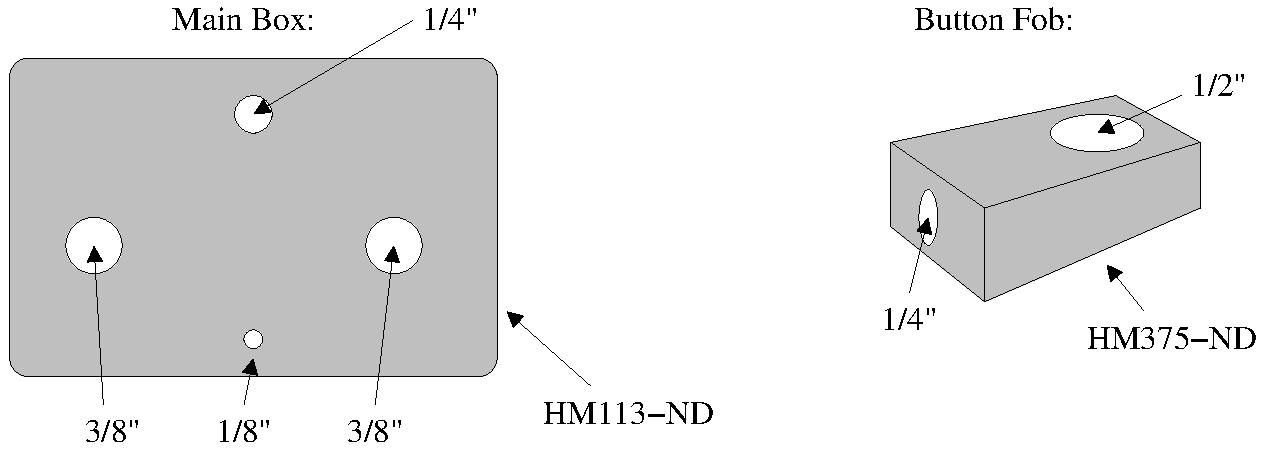
\includegraphics[width=0.8\columnwidth]
{figs-pump/pump-box-v1-mech-notitle.pdf}
\end{center}
\caption{Pump control box cutouts.}
\label{fig-pumpbox-boxes}
\end{figure}

\begin{table}[h]
\begin{center}
\begin{tabular}{llr}
\hline
\textbf{Item} & \textbf{Digikey p/n} & \textbf{Quantity} \\
\hline
box 3.25x2.25x1.5''		& HM113-ND	& 1	\\
box 2x1.5.0.75''		& HM375-ND	& 1	\\
transistor NPN TO-92		& 2N3904FS-ND	& 2	\\
resistor 1/4 W 10 kohm		& 10.0KXBK-ND	& 2	\\
resistor 1/4 W 3.3 kohm		& 3.3KXBK-ND	& 1	\\
proto board 1x1''		& 1568-1652-ND	& 1	\\
screw 4-40 nylon 1/4''		& H542-ND	& 1	\\
standoff nylon 4-40 F/F 1/2''	& 36-1902C-ND	& 1	\\
screw metal 4-40 3/8''		& HM1456-ND	& 1	\\
jack BNC panel mount		& ARFX1064-ND	& 1	\\
jack audio 1/4'' stereo panel	& SC1563-ND	& 1	\\
plug audio 1/4'' stereo		& SC1081-ND	& 1	\\
jack audio 3.5mm mono panel	& SC1455-ND	& 2	\\
cable audio 3.5mm M/M 10'	& TL634-ND	& 1	\\
button spst-no panel mount	& CW158-ND	& 1	\\
cable M12 rev key to wire	& $^\dagger$	& 1	\\
\hline
\multicolumn{3}{p{0.8\columnwidth}}
{$^\dagger$Sold by LMI as part number 48414; may be sourced more cheaply as
MEC-5FP-2M from www.mencom.com. These have a ``5 pole reverse-keyed'' M12
connector.} \\
\end{tabular}
\end{center}
\caption{Pump control box bill of materials.}
\label{tab-pumpbox-bom}
\end{table}

\clearpage
\section{Pump Cable Plug}
\label{sect-pumpbox-plug}

Assembly steps for the pump cable plug are shown below. Use of
$\frac{1}{8}$'' heat shrink tubing is strongly recommended to avoid shorts
within the plug housing.

\begin{itemize}
%
\item Trim wires to appropriate lengths, and feed cable through backshell.

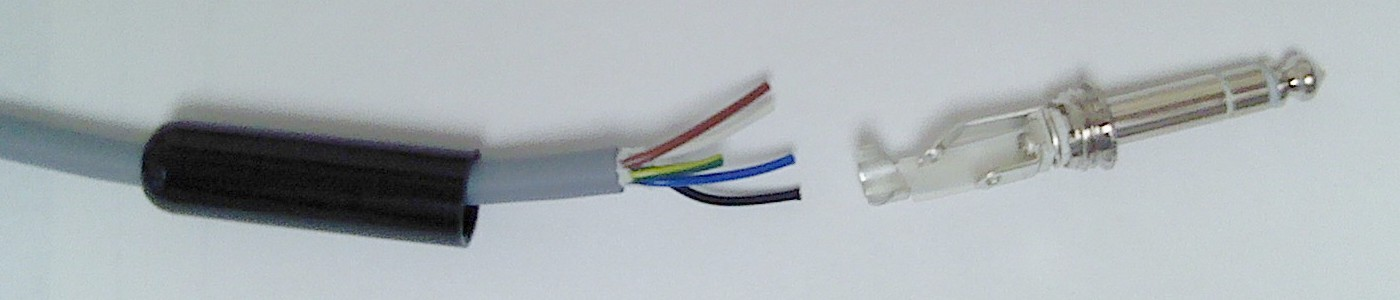
\includegraphics[width=0.8\columnwidth]
{photos/pump-box-20181030/plug-started.jpg}

\item Cap green wire with heat shrink, twist brown and white wires together
and tin, tin blue wire, solder resistor to black wire.

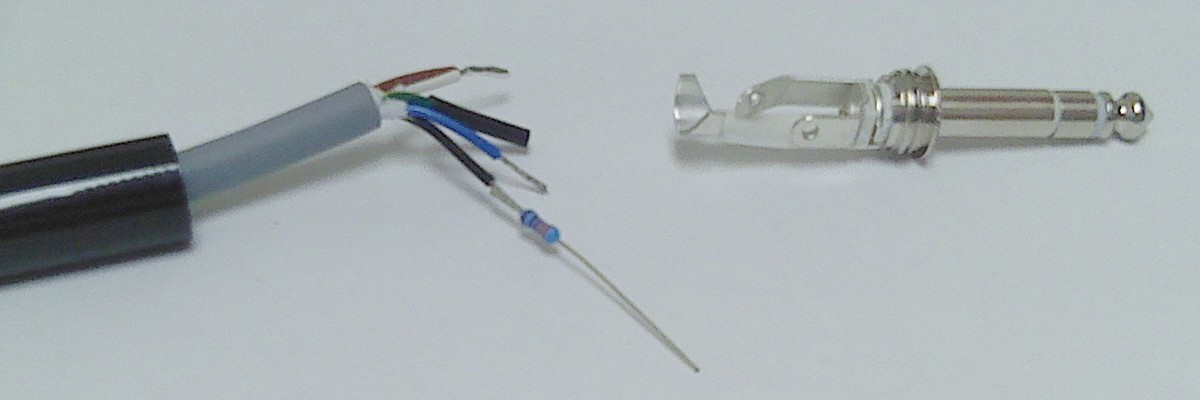
\includegraphics[width=0.8\columnwidth]
{photos/pump-box-20181030/plug-midway.jpg}

\item Cover resistor connection with heat shrink, solder blue wire,
resistor lead, and brown/white wire pair to appropriate lugs.

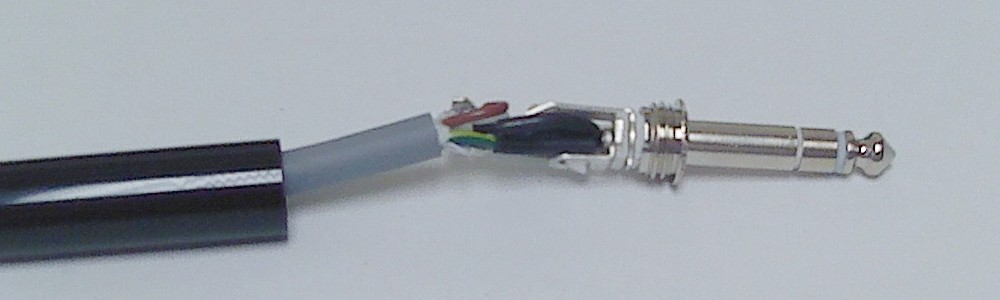
\includegraphics[width=0.8\columnwidth]
{photos/pump-box-20181030/plug-done.jpg}

\item Crimp collar around wires and screw backshell on to plug.

\textbf{NOTE} - ideally the wires would be short enough that the collar is
crimped to the jacket rather than to the wire bundle.
%
\end{itemize}

\clearpage
\section{Circuit Board}
\label{sect-pumpbox-board}

Assembly steps for the circuit board are shown below. The prototyping board
trace pattern and one possible layout are shown in Figure
\ref{fig-pumpbox-protoboard}.

\begin{figure}
\begin{center}
\begin{tabular}{ccc}
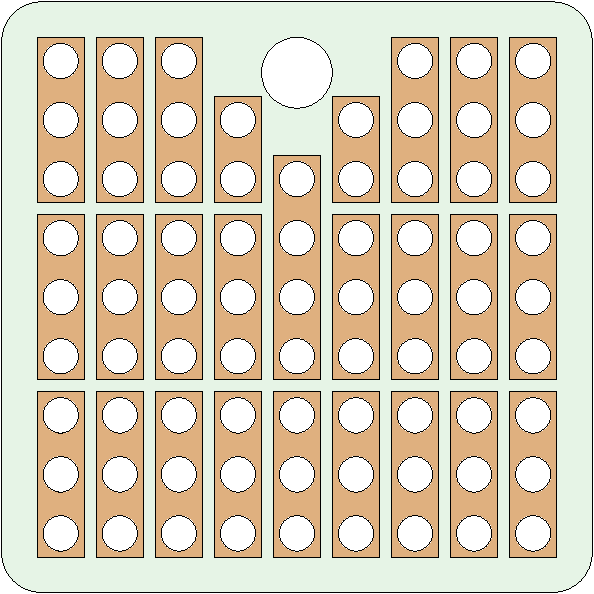
\includegraphics[height=2in]
{figs-pump/pump-box-v1-breadboard.pdf}
& ~ &
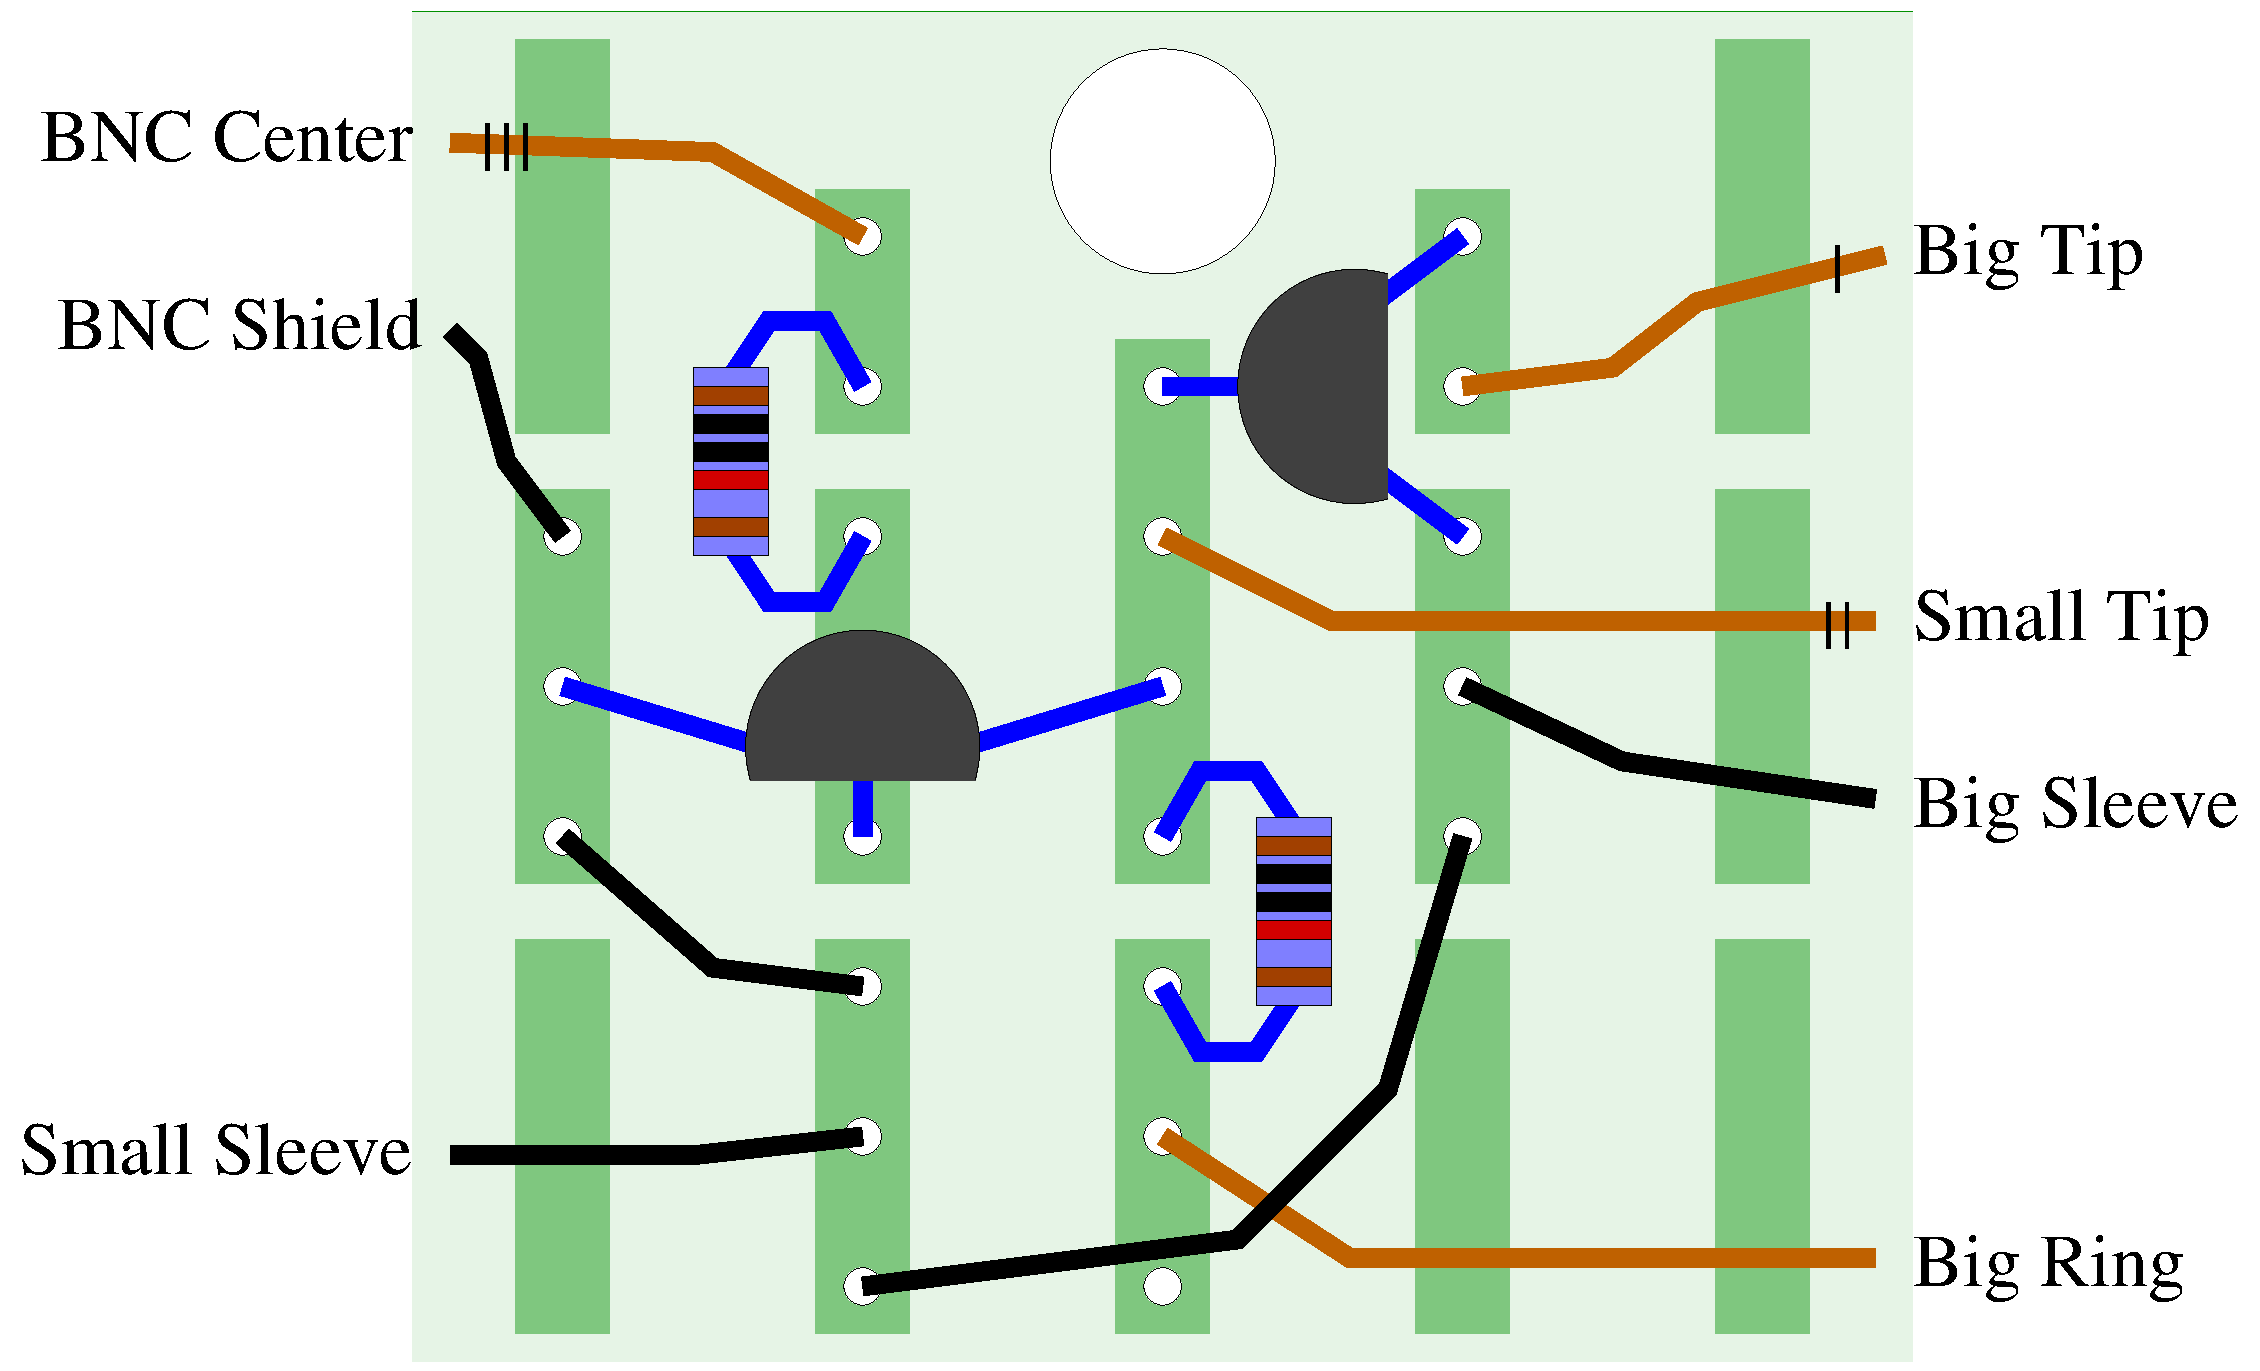
\includegraphics[height=2in]
{figs-pump/pump-box-v1-bblayout.pdf}
\\
\end{tabular}
\end{center}
\caption{Prototyping board and one possible pump control circuit layout.}
\label{fig-pumpbox-protoboard}
\end{figure}

\begin{itemize}
%
\item Solder transistors and resistors.

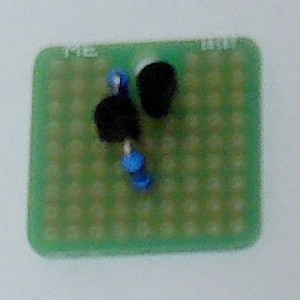
\includegraphics[height=2in]
{photos/pump-box-20181112/board-comps.jpg}

\item Solder signal and power wires. Marking is encouraged to keep track
of which are which.

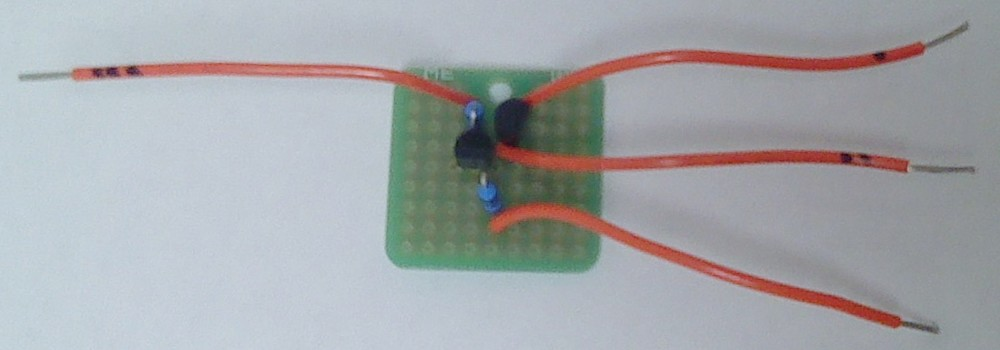
\includegraphics[height=2in]
{photos/pump-box-20181112/board-orange.jpg}

\clearpage
\item Solder ground wires.

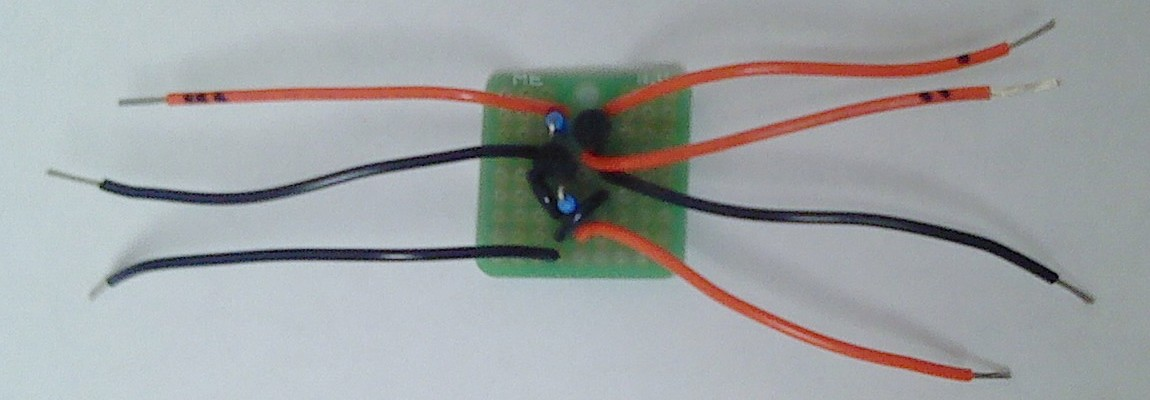
\includegraphics[height=2in]
{photos/pump-box-20181112/board-black.jpg}

\item Solder jacks to wires. Make sure to thread BNC hardware over the BNC
signal wire and to insert the BNC connector in the faceplate before soldering.

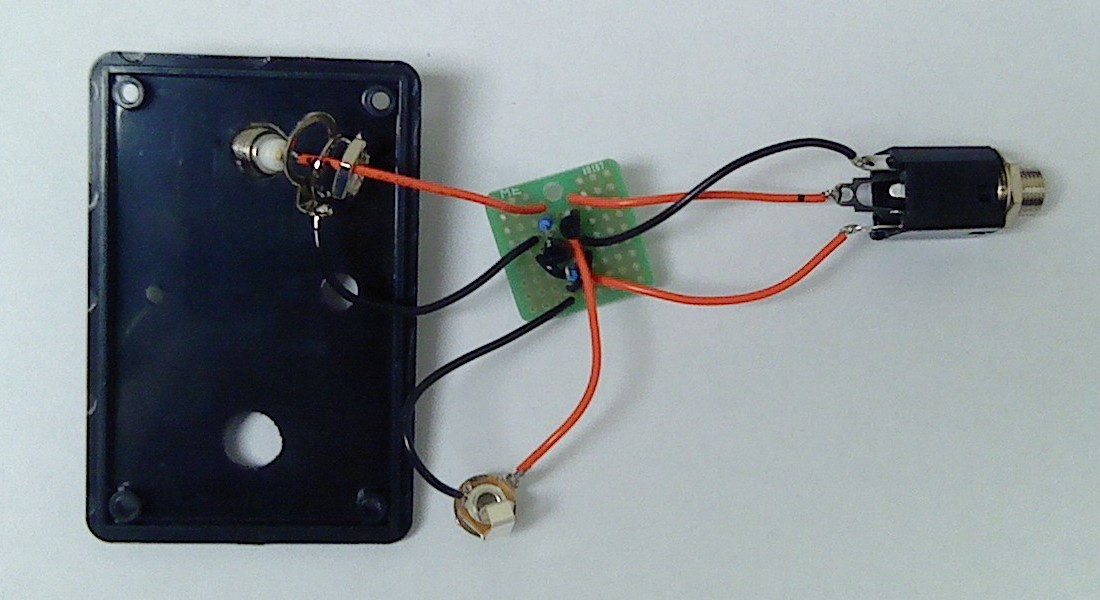
\includegraphics[height=3in]
{photos/pump-box-20181112/board-conns.jpg}

\item Screw circuit board to faceplate.

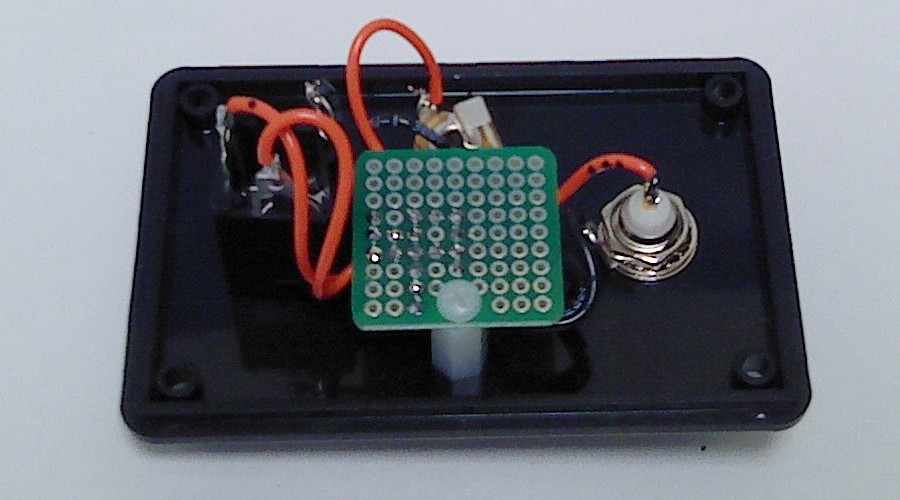
\includegraphics[height=2in]
{photos/pump-box-20181030/board-done.jpg}
%
\end{itemize}

%
% This is the end of the file.


\end{document}

%
% This is the end of the file.
